% Options for packages loaded elsewhere
\PassOptionsToPackage{unicode}{hyperref}
\PassOptionsToPackage{hyphens}{url}
%
\documentclass[
]{article}
\usepackage{lmodern}
\usepackage{amssymb,amsmath}
\usepackage{ifxetex,ifluatex}
\ifnum 0\ifxetex 1\fi\ifluatex 1\fi=0 % if pdftex
  \usepackage[T1]{fontenc}
  \usepackage[utf8]{inputenc}
  \usepackage{textcomp} % provide euro and other symbols
\else % if luatex or xetex
  \usepackage{unicode-math}
  \defaultfontfeatures{Scale=MatchLowercase}
  \defaultfontfeatures[\rmfamily]{Ligatures=TeX,Scale=1}
\fi
% Use upquote if available, for straight quotes in verbatim environments
\IfFileExists{upquote.sty}{\usepackage{upquote}}{}
\IfFileExists{microtype.sty}{% use microtype if available
  \usepackage[]{microtype}
  \UseMicrotypeSet[protrusion]{basicmath} % disable protrusion for tt fonts
}{}
\makeatletter
\@ifundefined{KOMAClassName}{% if non-KOMA class
  \IfFileExists{parskip.sty}{%
    \usepackage{parskip}
  }{% else
    \setlength{\parindent}{0pt}
    \setlength{\parskip}{6pt plus 2pt minus 1pt}}
}{% if KOMA class
  \KOMAoptions{parskip=half}}
\makeatother
\usepackage{xcolor}
\IfFileExists{xurl.sty}{\usepackage{xurl}}{} % add URL line breaks if available
\IfFileExists{bookmark.sty}{\usepackage{bookmark}}{\usepackage{hyperref}}
\hypersetup{
  pdftitle={04 Ontology Visualization},
  pdfauthor={Thomas J. Brailey},
  hidelinks,
  pdfcreator={LaTeX via pandoc}}
\urlstyle{same} % disable monospaced font for URLs
\usepackage[margin=1in]{geometry}
\usepackage{color}
\usepackage{fancyvrb}
\newcommand{\VerbBar}{|}
\newcommand{\VERB}{\Verb[commandchars=\\\{\}]}
\DefineVerbatimEnvironment{Highlighting}{Verbatim}{commandchars=\\\{\}}
% Add ',fontsize=\small' for more characters per line
\usepackage{framed}
\definecolor{shadecolor}{RGB}{248,248,248}
\newenvironment{Shaded}{\begin{snugshade}}{\end{snugshade}}
\newcommand{\AlertTok}[1]{\textcolor[rgb]{0.94,0.16,0.16}{#1}}
\newcommand{\AnnotationTok}[1]{\textcolor[rgb]{0.56,0.35,0.01}{\textbf{\textit{#1}}}}
\newcommand{\AttributeTok}[1]{\textcolor[rgb]{0.77,0.63,0.00}{#1}}
\newcommand{\BaseNTok}[1]{\textcolor[rgb]{0.00,0.00,0.81}{#1}}
\newcommand{\BuiltInTok}[1]{#1}
\newcommand{\CharTok}[1]{\textcolor[rgb]{0.31,0.60,0.02}{#1}}
\newcommand{\CommentTok}[1]{\textcolor[rgb]{0.56,0.35,0.01}{\textit{#1}}}
\newcommand{\CommentVarTok}[1]{\textcolor[rgb]{0.56,0.35,0.01}{\textbf{\textit{#1}}}}
\newcommand{\ConstantTok}[1]{\textcolor[rgb]{0.00,0.00,0.00}{#1}}
\newcommand{\ControlFlowTok}[1]{\textcolor[rgb]{0.13,0.29,0.53}{\textbf{#1}}}
\newcommand{\DataTypeTok}[1]{\textcolor[rgb]{0.13,0.29,0.53}{#1}}
\newcommand{\DecValTok}[1]{\textcolor[rgb]{0.00,0.00,0.81}{#1}}
\newcommand{\DocumentationTok}[1]{\textcolor[rgb]{0.56,0.35,0.01}{\textbf{\textit{#1}}}}
\newcommand{\ErrorTok}[1]{\textcolor[rgb]{0.64,0.00,0.00}{\textbf{#1}}}
\newcommand{\ExtensionTok}[1]{#1}
\newcommand{\FloatTok}[1]{\textcolor[rgb]{0.00,0.00,0.81}{#1}}
\newcommand{\FunctionTok}[1]{\textcolor[rgb]{0.00,0.00,0.00}{#1}}
\newcommand{\ImportTok}[1]{#1}
\newcommand{\InformationTok}[1]{\textcolor[rgb]{0.56,0.35,0.01}{\textbf{\textit{#1}}}}
\newcommand{\KeywordTok}[1]{\textcolor[rgb]{0.13,0.29,0.53}{\textbf{#1}}}
\newcommand{\NormalTok}[1]{#1}
\newcommand{\OperatorTok}[1]{\textcolor[rgb]{0.81,0.36,0.00}{\textbf{#1}}}
\newcommand{\OtherTok}[1]{\textcolor[rgb]{0.56,0.35,0.01}{#1}}
\newcommand{\PreprocessorTok}[1]{\textcolor[rgb]{0.56,0.35,0.01}{\textit{#1}}}
\newcommand{\RegionMarkerTok}[1]{#1}
\newcommand{\SpecialCharTok}[1]{\textcolor[rgb]{0.00,0.00,0.00}{#1}}
\newcommand{\SpecialStringTok}[1]{\textcolor[rgb]{0.31,0.60,0.02}{#1}}
\newcommand{\StringTok}[1]{\textcolor[rgb]{0.31,0.60,0.02}{#1}}
\newcommand{\VariableTok}[1]{\textcolor[rgb]{0.00,0.00,0.00}{#1}}
\newcommand{\VerbatimStringTok}[1]{\textcolor[rgb]{0.31,0.60,0.02}{#1}}
\newcommand{\WarningTok}[1]{\textcolor[rgb]{0.56,0.35,0.01}{\textbf{\textit{#1}}}}
\usepackage{graphicx,grffile}
\makeatletter
\def\maxwidth{\ifdim\Gin@nat@width>\linewidth\linewidth\else\Gin@nat@width\fi}
\def\maxheight{\ifdim\Gin@nat@height>\textheight\textheight\else\Gin@nat@height\fi}
\makeatother
% Scale images if necessary, so that they will not overflow the page
% margins by default, and it is still possible to overwrite the defaults
% using explicit options in \includegraphics[width, height, ...]{}
\setkeys{Gin}{width=\maxwidth,height=\maxheight,keepaspectratio}
% Set default figure placement to htbp
\makeatletter
\def\fps@figure{htbp}
\makeatother
\setlength{\emergencystretch}{3em} % prevent overfull lines
\providecommand{\tightlist}{%
  \setlength{\itemsep}{0pt}\setlength{\parskip}{0pt}}
\setcounter{secnumdepth}{-\maxdimen} % remove section numbering

\title{04 Ontology Visualization}
\author{Thomas J. Brailey}
\date{29/09/2019}

\begin{document}
\maketitle

{
\setcounter{tocdepth}{2}
\tableofcontents
}
\hypertarget{load-data}{%
\section{Load data}\label{load-data}}

\begin{Shaded}
\begin{Highlighting}[]
\CommentTok{# Read in excel file }
\NormalTok{files <-}\StringTok{ }\KeywordTok{list.files}\NormalTok{(}\KeywordTok{paste0}\NormalTok{(here}\OperatorTok{::}\KeywordTok{here}\NormalTok{(), }\StringTok{"/data/"}\NormalTok{), }
                    \StringTok{"tjbrailey_psp_ontology.xlsx"}\NormalTok{, }
                    \DataTypeTok{full.names =} \OtherTok{TRUE}
\NormalTok{                    )}
\NormalTok{files <-}\StringTok{ }\NormalTok{files[}\DecValTok{2}\NormalTok{]}

\NormalTok{read_excel_allsheets <-}\StringTok{ }\ControlFlowTok{function}\NormalTok{(filename) \{ }
\NormalTok{  sheets <-}\StringTok{ }\NormalTok{readxl}\OperatorTok{::}\KeywordTok{excel_sheets}\NormalTok{(filename) }
\NormalTok{  x <-}\StringTok{ }\KeywordTok{lapply}\NormalTok{(sheets, }\ControlFlowTok{function}\NormalTok{(X) readxl}\OperatorTok{::}\KeywordTok{read_excel}\NormalTok{(filename, }\DataTypeTok{sheet =}\NormalTok{ X)) }
  \KeywordTok{names}\NormalTok{(x) <-}\StringTok{ }\NormalTok{sheets }
\NormalTok{  x }
\NormalTok{\} }

\NormalTok{out <-}\StringTok{ }\KeywordTok{lapply}\NormalTok{(files, read_excel_allsheets)}
\KeywordTok{basename}\NormalTok{(files)}
\end{Highlighting}
\end{Shaded}

\begin{verbatim}
## [1] "tjbrailey_psp_ontology.xlsx"
\end{verbatim}

\begin{Shaded}
\begin{Highlighting}[]
\NormalTok{psp_ont <-}\StringTok{ }\NormalTok{out[[}\DecValTok{1}\NormalTok{]]}\OperatorTok{$}\NormalTok{Sheet1}
\NormalTok{psp_ont <-}\StringTok{ }\NormalTok{dplyr}\OperatorTok{::}\KeywordTok{as_data_frame}\NormalTok{(psp_ont)}
\end{Highlighting}
\end{Shaded}

\begin{verbatim}
## Warning: `as_data_frame()` is deprecated, use `as_tibble()` (but mind the new semantics).
## This warning is displayed once per session.
\end{verbatim}

\begin{Shaded}
\begin{Highlighting}[]
\CommentTok{# Select relevant variables}
\NormalTok{psp_ont_prep <-}\StringTok{ }\NormalTok{psp_ont }\OperatorTok
\StringTok{  }\NormalTok{dplyr}\OperatorTok{::}\KeywordTok{select}\NormalTok{(child_}\DecValTok{0}\NormalTok{,}
\NormalTok{                child_}\DecValTok{1}\NormalTok{,}
\NormalTok{                provisions)}

\CommentTok{# Do the same for regional autonomy}
\NormalTok{reg_aut_ont <-}\StringTok{ }\NormalTok{out[[}\DecValTok{1}\NormalTok{]]}\OperatorTok{$}\NormalTok{Sheet2}
\NormalTok{reg_aut_ont <-}\StringTok{ }\NormalTok{dplyr}\OperatorTok{::}\KeywordTok{as_data_frame}\NormalTok{(reg_aut_ont)}
\end{Highlighting}
\end{Shaded}

\hypertarget{define-hierarchy}{%
\section{Define hierarchy}\label{define-hierarchy}}

\begin{Shaded}
\begin{Highlighting}[]
\CommentTok{# Generate pathString as new column}
\NormalTok{psp_ont_prep}\OperatorTok{$}\NormalTok{pathString <-}\StringTok{ }\KeywordTok{paste}\NormalTok{(}\StringTok{"Power Sharing Provision"}\NormalTok{,}
\NormalTok{                             psp_ont_prep}\OperatorTok{$}\NormalTok{child_}\DecValTok{0}\NormalTok{,}
\NormalTok{                             psp_ont_prep}\OperatorTok{$}\NormalTok{child_}\DecValTok{1}\NormalTok{,}
\NormalTok{                             psp_ont_prep}\OperatorTok{$}\NormalTok{provisions,}
                             \DataTypeTok{sep =} \StringTok{"|"}\NormalTok{)}

\CommentTok{# Create list }
\NormalTok{psp_tree <-}\StringTok{ }\NormalTok{data.tree}\OperatorTok{::}\KeywordTok{as.Node}\NormalTok{(psp_ont_prep, }\DataTypeTok{pathDelimiter =} \StringTok{"|"}\NormalTok{)}
\KeywordTok{print}\NormalTok{(psp_tree, }\DataTypeTok{limit =} \DecValTok{15}\NormalTok{)}
\end{Highlighting}
\end{Shaded}

\begin{verbatim}
##                                  levelName
## 1  Power Sharing Provision                
## 2   ¦--political system                   
## 3   ¦   ¦--general consocilationalism     
## 4   ¦   ¦   ¦--grand coalition            
## 5   ¦   ¦   ¦--mutual veto                
## 6   ¦   ¦   ¦--proportionality            
## 7   ¦   ¦   ¦--segmental autonomy         
## 8   ¦   ¦   ¦--coalition cabinets         
## 9   ¦   ¦   ¦--bicameralism               
## 10  ¦   ¦   ¦--proportional representation
## 11  ¦   ¦   ¦--organized interest groups  
## 12  ¦   ¦   ¦--rigid constitution         
## 13  ¦   ¦   ¦--judicial review            
## 14  ¦   ¦   ¦--direct democracy           
## 15  ¦   ¦   °--... 7 nodes w/ 0 sub       
## 16  ¦   °--... 5 nodes w/ 26 sub          
## 17  °--... 2 nodes w/ 85 sub
\end{verbatim}

\begin{Shaded}
\begin{Highlighting}[]
\CommentTok{# Do the same for regional autonomy only }
\NormalTok{reg_aut_ont}\OperatorTok{$}\NormalTok{pathString <-}\StringTok{ }\KeywordTok{paste}\NormalTok{(reg_aut_ont}\OperatorTok{$}\NormalTok{provision,}
\NormalTok{                             reg_aut_ont}\OperatorTok{$}\NormalTok{concept,}
\NormalTok{                             reg_aut_ont}\OperatorTok{$}\NormalTok{citation,}
                             \DataTypeTok{sep =} \StringTok{"|"}\NormalTok{)}
\NormalTok{reg_aut_tree <-}\StringTok{ }\NormalTok{data.tree}\OperatorTok{::}\KeywordTok{as.Node}\NormalTok{(reg_aut_ont, }\DataTypeTok{pathDelimiter =} \StringTok{"|"}\NormalTok{)}
\KeywordTok{print}\NormalTok{(reg_aut_tree, }\DataTypeTok{limit =} \DecValTok{15}\NormalTok{)}
\end{Highlighting}
\end{Shaded}

\begin{verbatim}
##                                                                  levelName
## 1  regional autonomy                                                      
## 2   ¦--partition                                                          
## 3   ¦   °--Berg, Eiki, and Guy Ben-Porat. (2008).                         
## 4   ¦--territorial power-sharing                                          
## 5   ¦   °--Hartzell, C., & Hoddie, M. (2007).                             
## 6   ¦--dispersive power-sharing                                           
## 7   ¦   °--Strøm, K. W., Gates, S., Graham, B. A. T., & Strand, H. (2017).
## 8   ¦--complex power-sharing                                              
## 9   ¦   °--Wolff, Stefan. (2009).                                         
## 10  ¦--vertical power-sharing                                             
## 11  ¦   °--Charron, N. (2009).                                            
## 12  ¦--consociationalism                                                  
## 13  ¦   °--Lijphart, A. (1969).                                           
## 14  °--corporate consociationalism                                        
## 15      °--O’Leary, Brendan. (2005).
\end{verbatim}

\hypertarget{visualizations}{%
\section{Visualizations}\label{visualizations}}

\begin{Shaded}
\begin{Highlighting}[]
\CommentTok{# Pepare list for visualization }
\NormalTok{psp_list <-}\StringTok{ }\NormalTok{data.tree}\OperatorTok{::}\KeywordTok{ToListExplicit}\NormalTok{(psp_tree, }\DataTypeTok{unname =} \OtherTok{TRUE}\NormalTok{)}
\NormalTok{psp_ontology_vis <-}\StringTok{ }\NormalTok{networkD3}\OperatorTok{::}\KeywordTok{diagonalNetwork}\NormalTok{(psp_list, }
                         \DataTypeTok{fontSize =} \DecValTok{14}\NormalTok{,}
                         \DataTypeTok{textColour =} \StringTok{"black"}\NormalTok{,}
                         \DataTypeTok{opacity =} \FloatTok{0.7}\NormalTok{,}
                         \DataTypeTok{width =} \DecValTok{1500}\NormalTok{,}
                         \DataTypeTok{height =} \DecValTok{1200}\NormalTok{)}
\CommentTok{# Visualize.}
\NormalTok{psp_ontology_vis}
\end{Highlighting}
\end{Shaded}

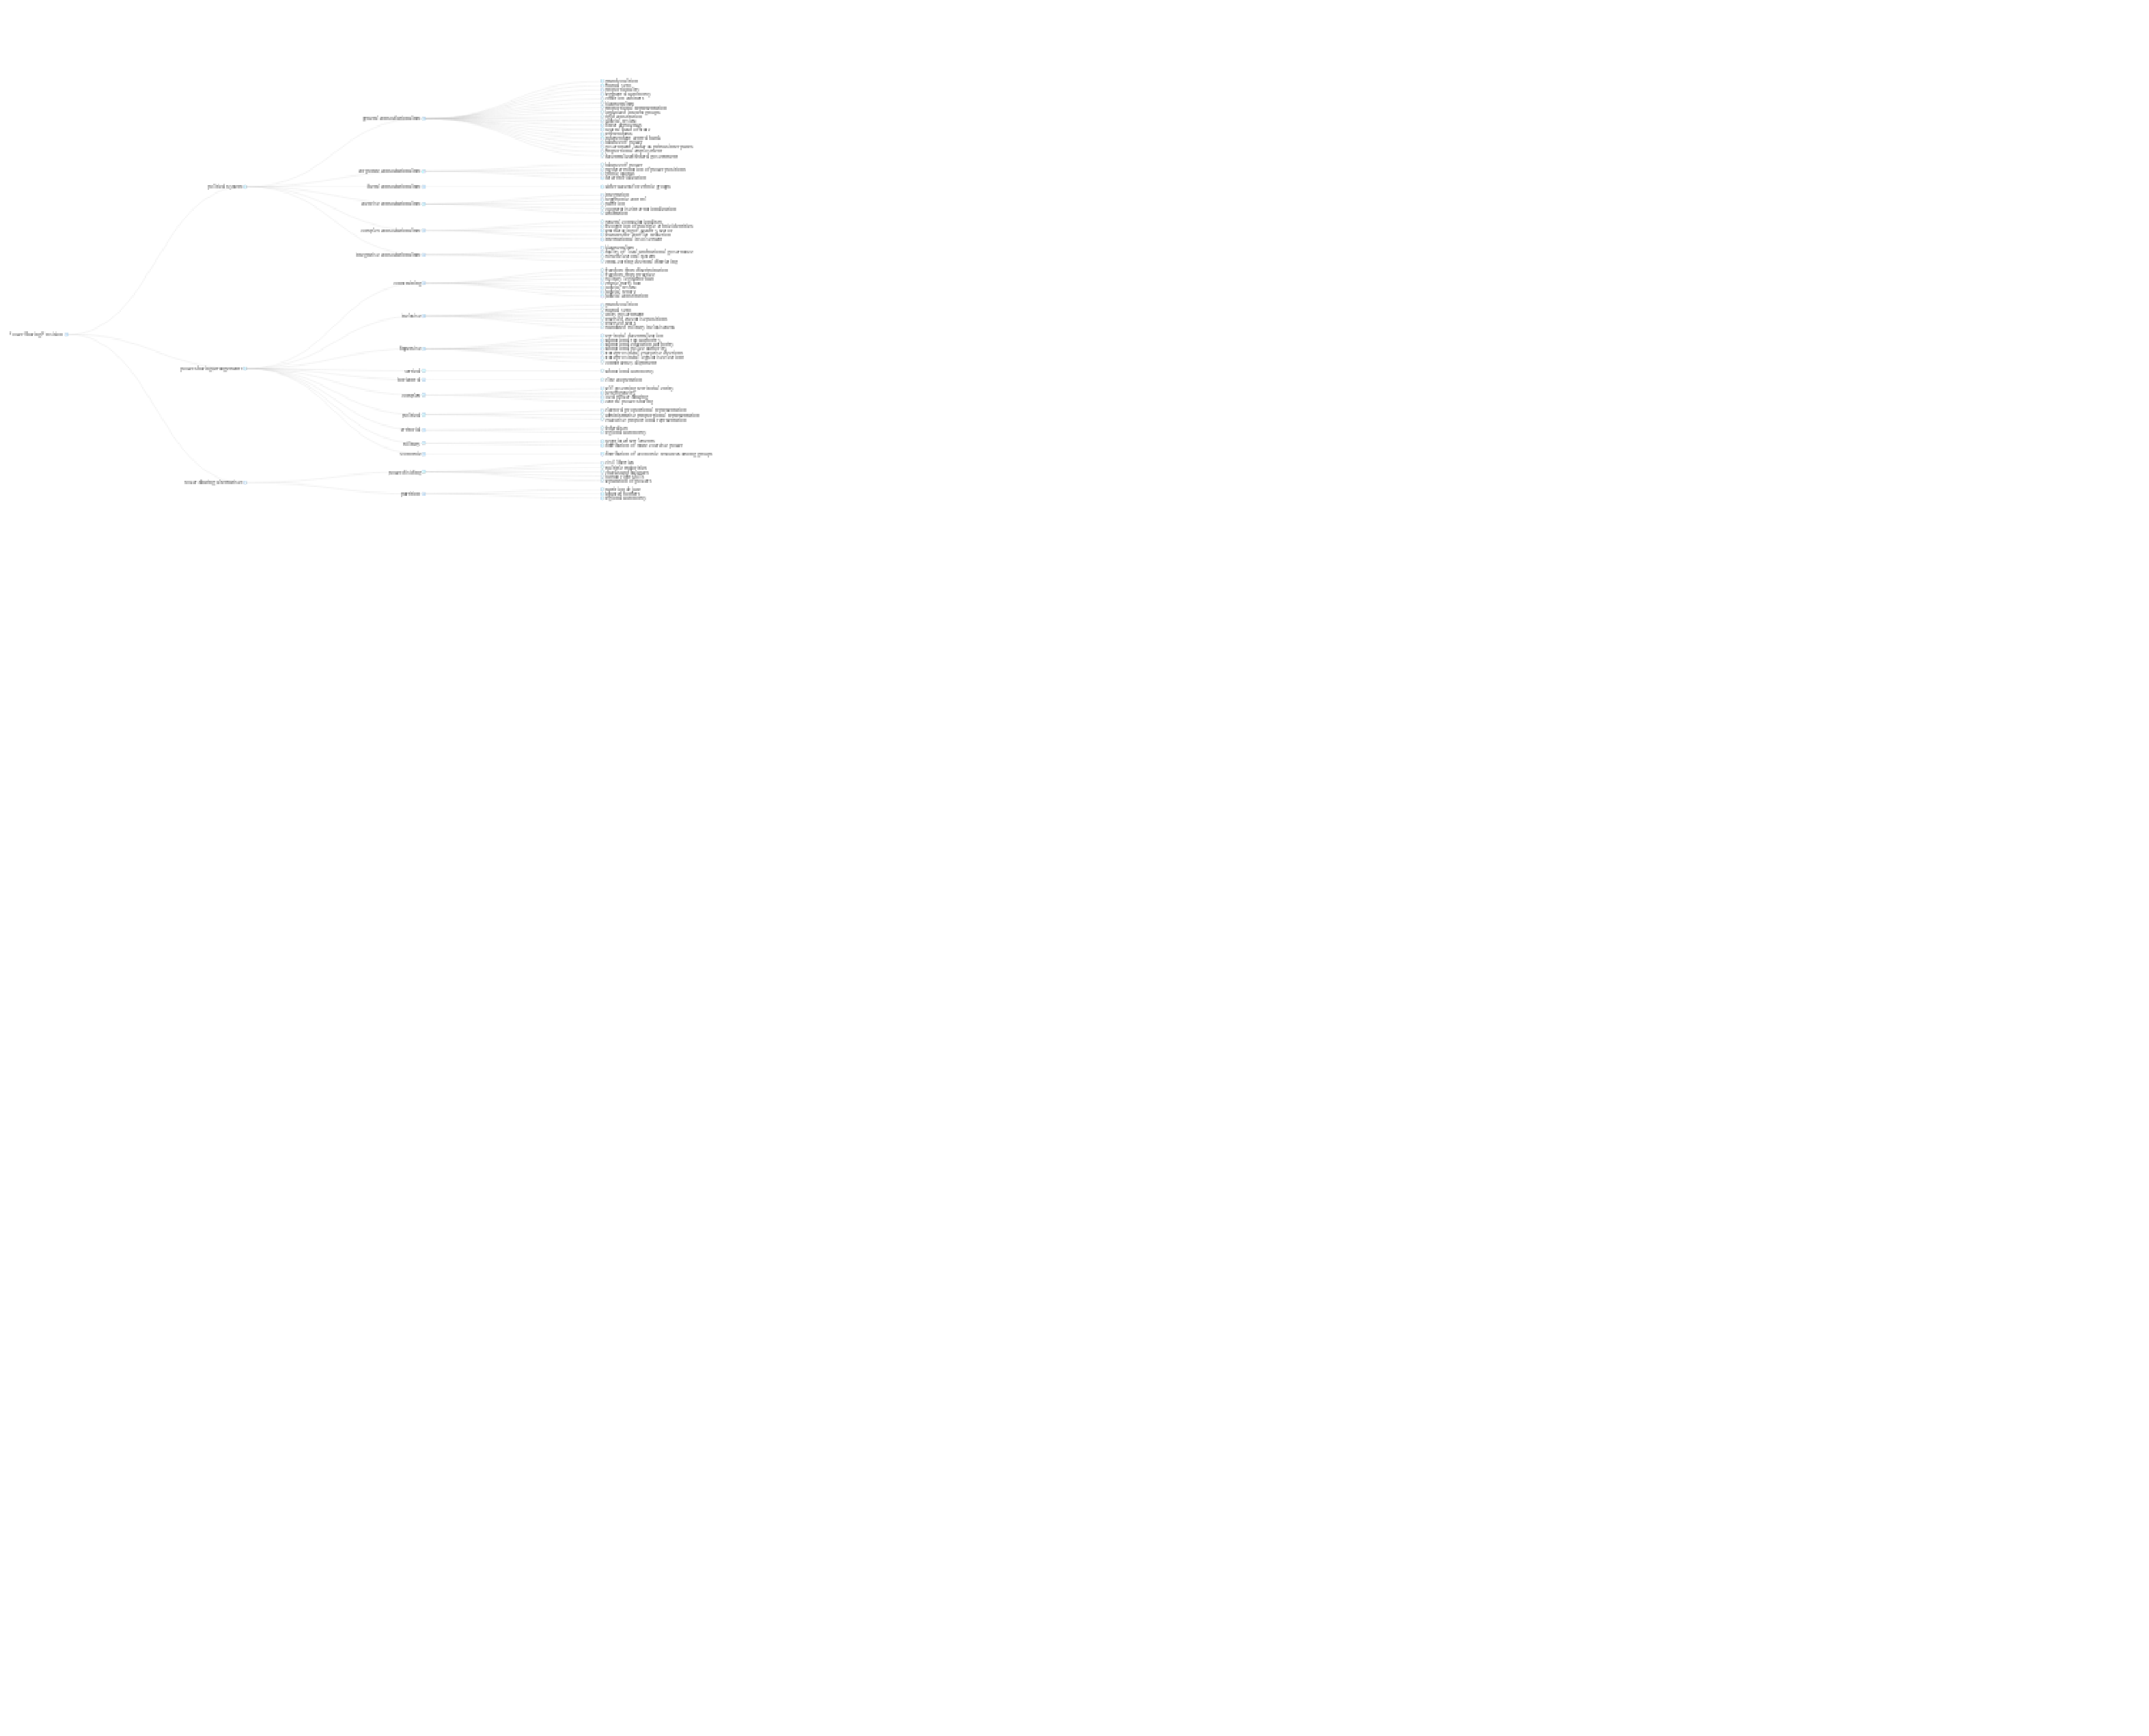
\includegraphics{04_tjbrailey_ontology_vis_files/figure-latex/unnamed-chunk-3-1.pdf}

\begin{Shaded}
\begin{Highlighting}[]
\CommentTok{# Do the same for regional autonomy}
\NormalTok{reg_aut_list <-}\StringTok{ }\NormalTok{data.tree}\OperatorTok{::}\KeywordTok{ToListExplicit}\NormalTok{(reg_aut_tree, }\DataTypeTok{unname =} \OtherTok{TRUE}\NormalTok{)}
\NormalTok{reg_aut_ontology_vis <-}\StringTok{ }\NormalTok{networkD3}\OperatorTok{::}\KeywordTok{diagonalNetwork}\NormalTok{(reg_aut_list, }
                         \DataTypeTok{fontSize =} \DecValTok{50}\NormalTok{,}
                         \DataTypeTok{textColour =} \StringTok{"black"}\NormalTok{,}
                         \DataTypeTok{opacity =} \FloatTok{0.7}\NormalTok{,}
                         \DataTypeTok{width =} \DecValTok{1500}\NormalTok{,}
                         \DataTypeTok{height =} \DecValTok{1200}\NormalTok{)}
\NormalTok{reg_aut_ontology_vis}
\end{Highlighting}
\end{Shaded}

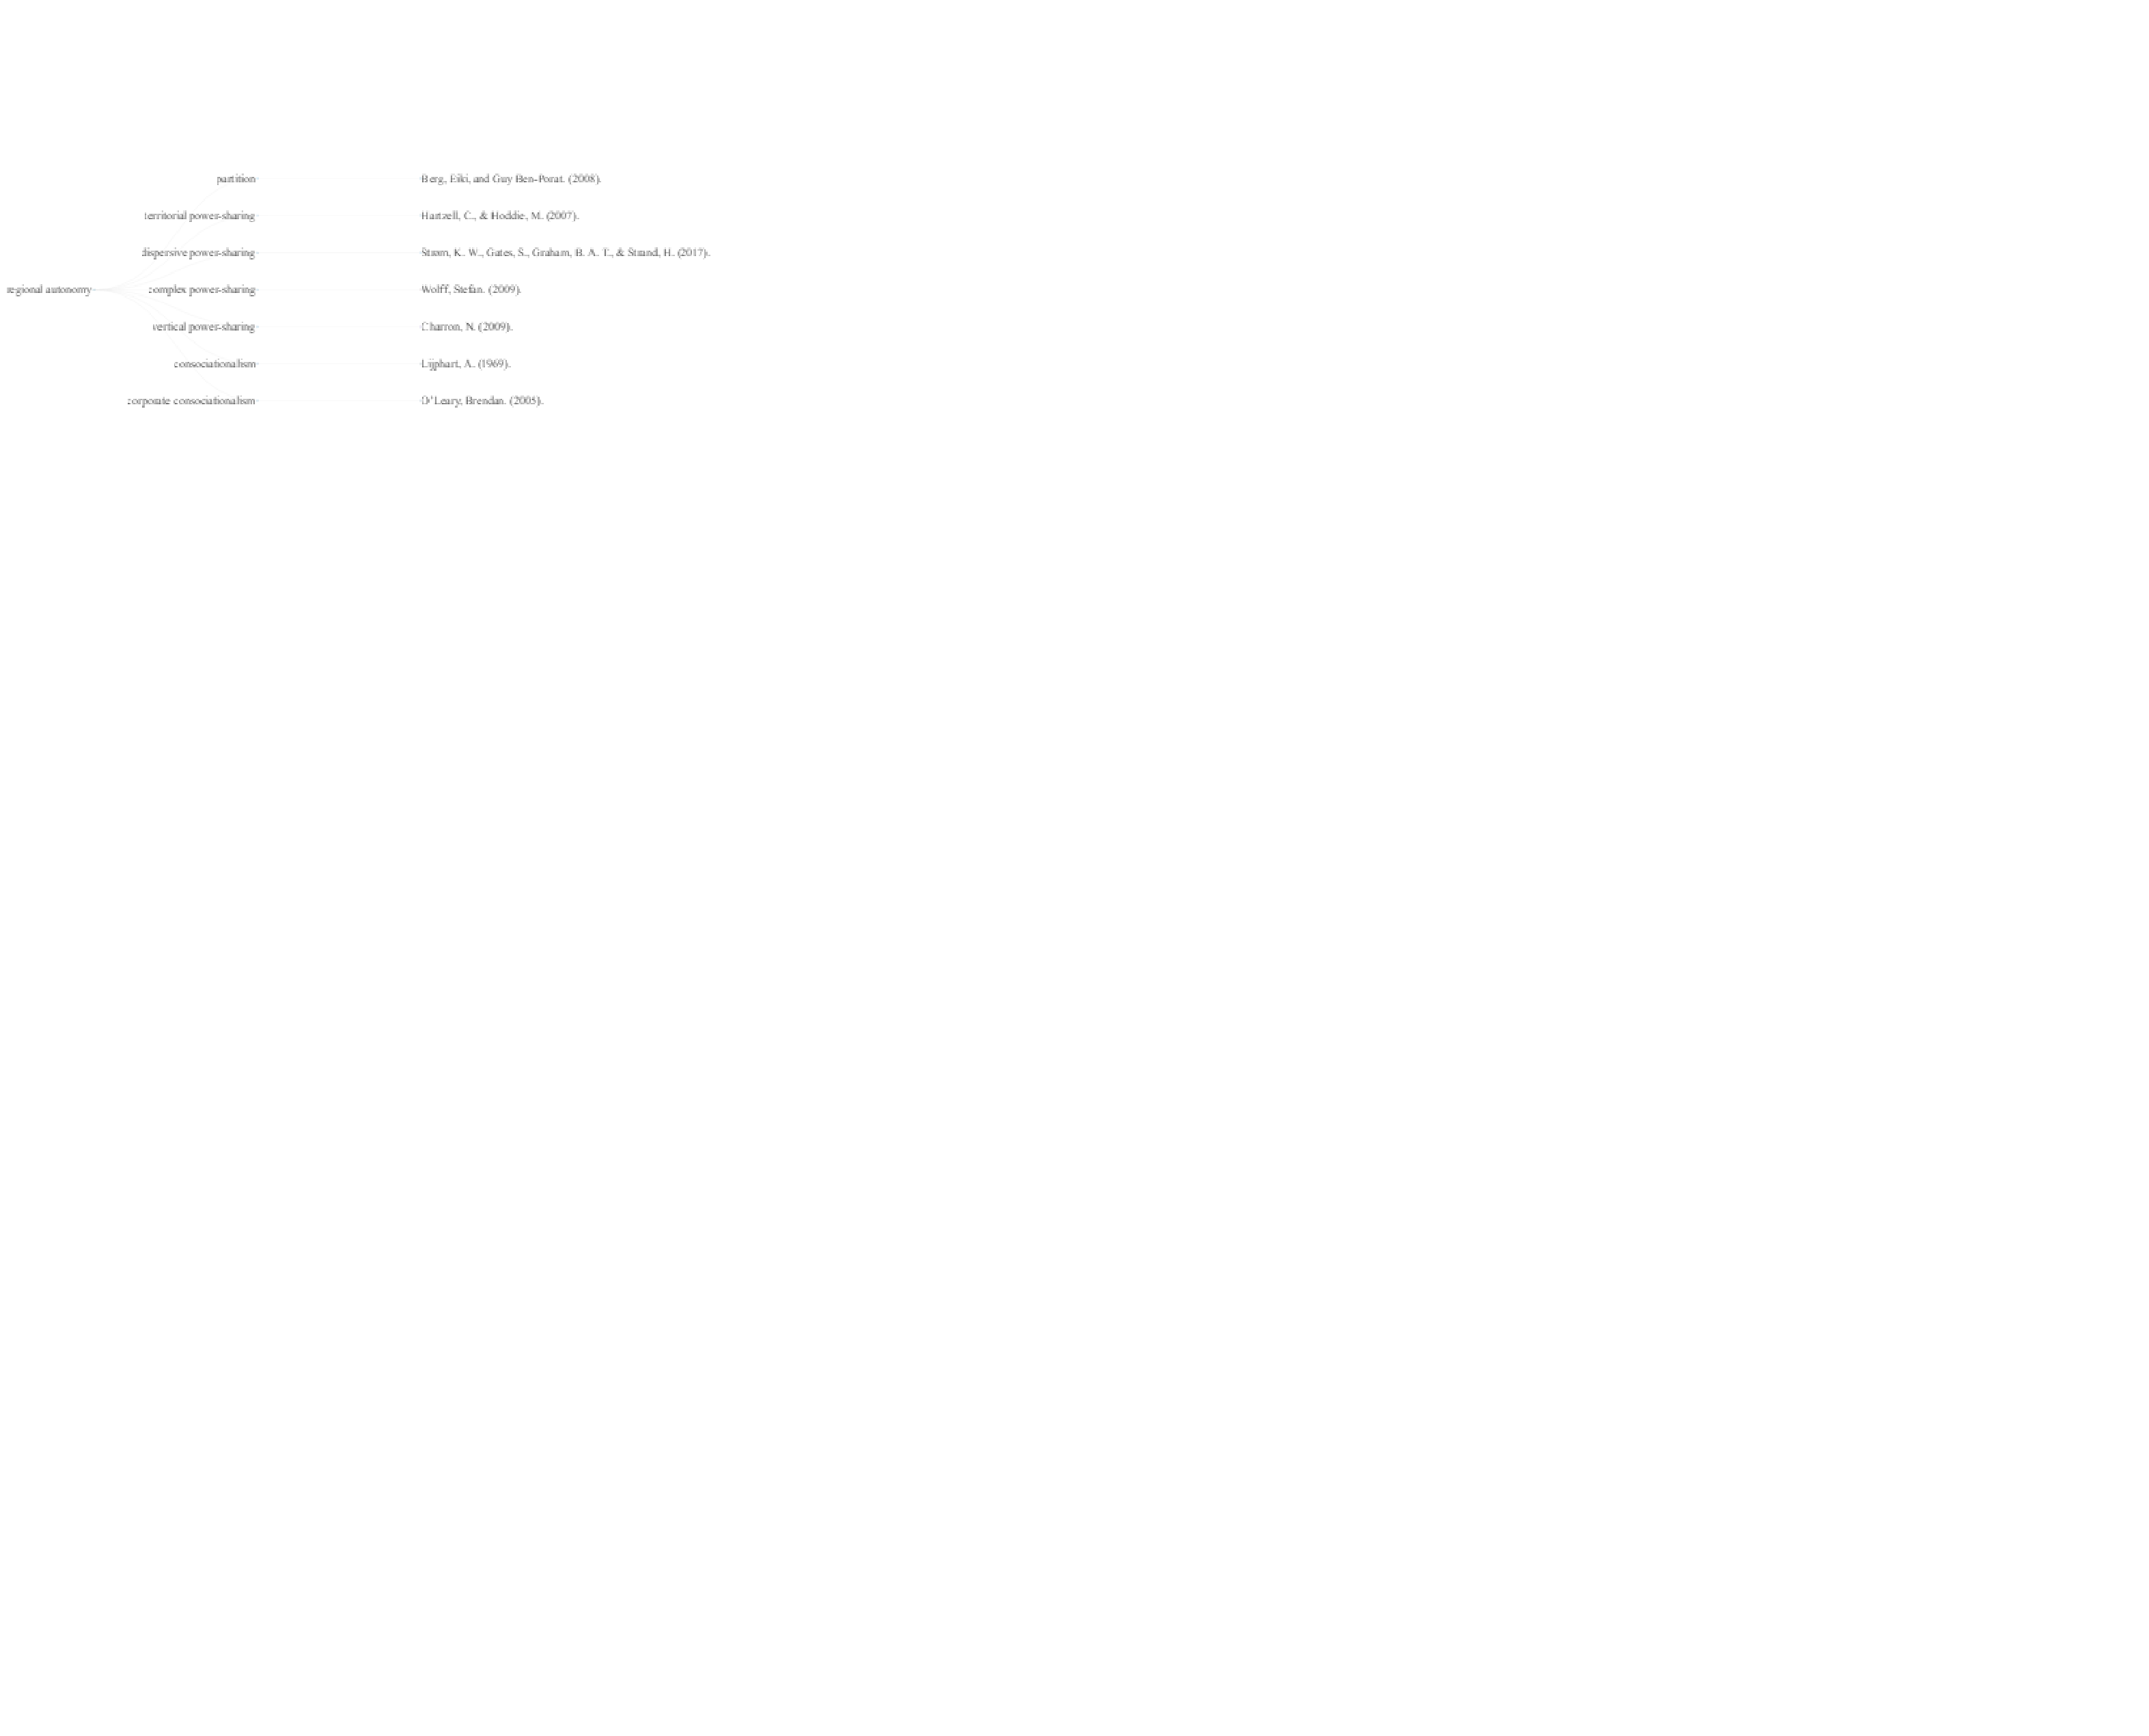
\includegraphics{04_tjbrailey_ontology_vis_files/figure-latex/unnamed-chunk-3-2.pdf}
\# Save

\end{document}
